\subsection{Телескоп}
\term{Телескоп}~--- оптическое устройство для наблюдения удаленных объектов. На данный момент существуют телескопы, для наблюдения во всех  диапазонах электро-магнитного излучения. По наблюдаемому диапазону телескопы делят на \imp{оптические} телескопы, \imp{радиотелескопы}, \imp{рентгеновские}телескопы и \imp{гамма-телескопы}. Каждый из классов в свою очередь содержит на множество подклассов. Поговорим подробнее про оптические телескопы.

Оптические телескопы по своей схеме делятся на три типа: \imp{рефлекторы} (диоптрические), \imp{рефракторы} (катаптрические) и \imp{катадиоптрические}.

\term{Рефрактор} (линзовый телескоп)~---  оптический телескоп, в котором для собирания света используется система линз.

\term{Рефлектор} (зеркальный телескоп)~---  оптический телескоп, светособирающий элемент~--- зеркало.

\term{Катадиоптрический} (зеркально-линзовый) \term{телескоп}~--- оптический телескоп, в котором используется как система линз, так и зеркал.

\begin{figure}
	\centering
	\begin{subfigure}{0.49\tw}
		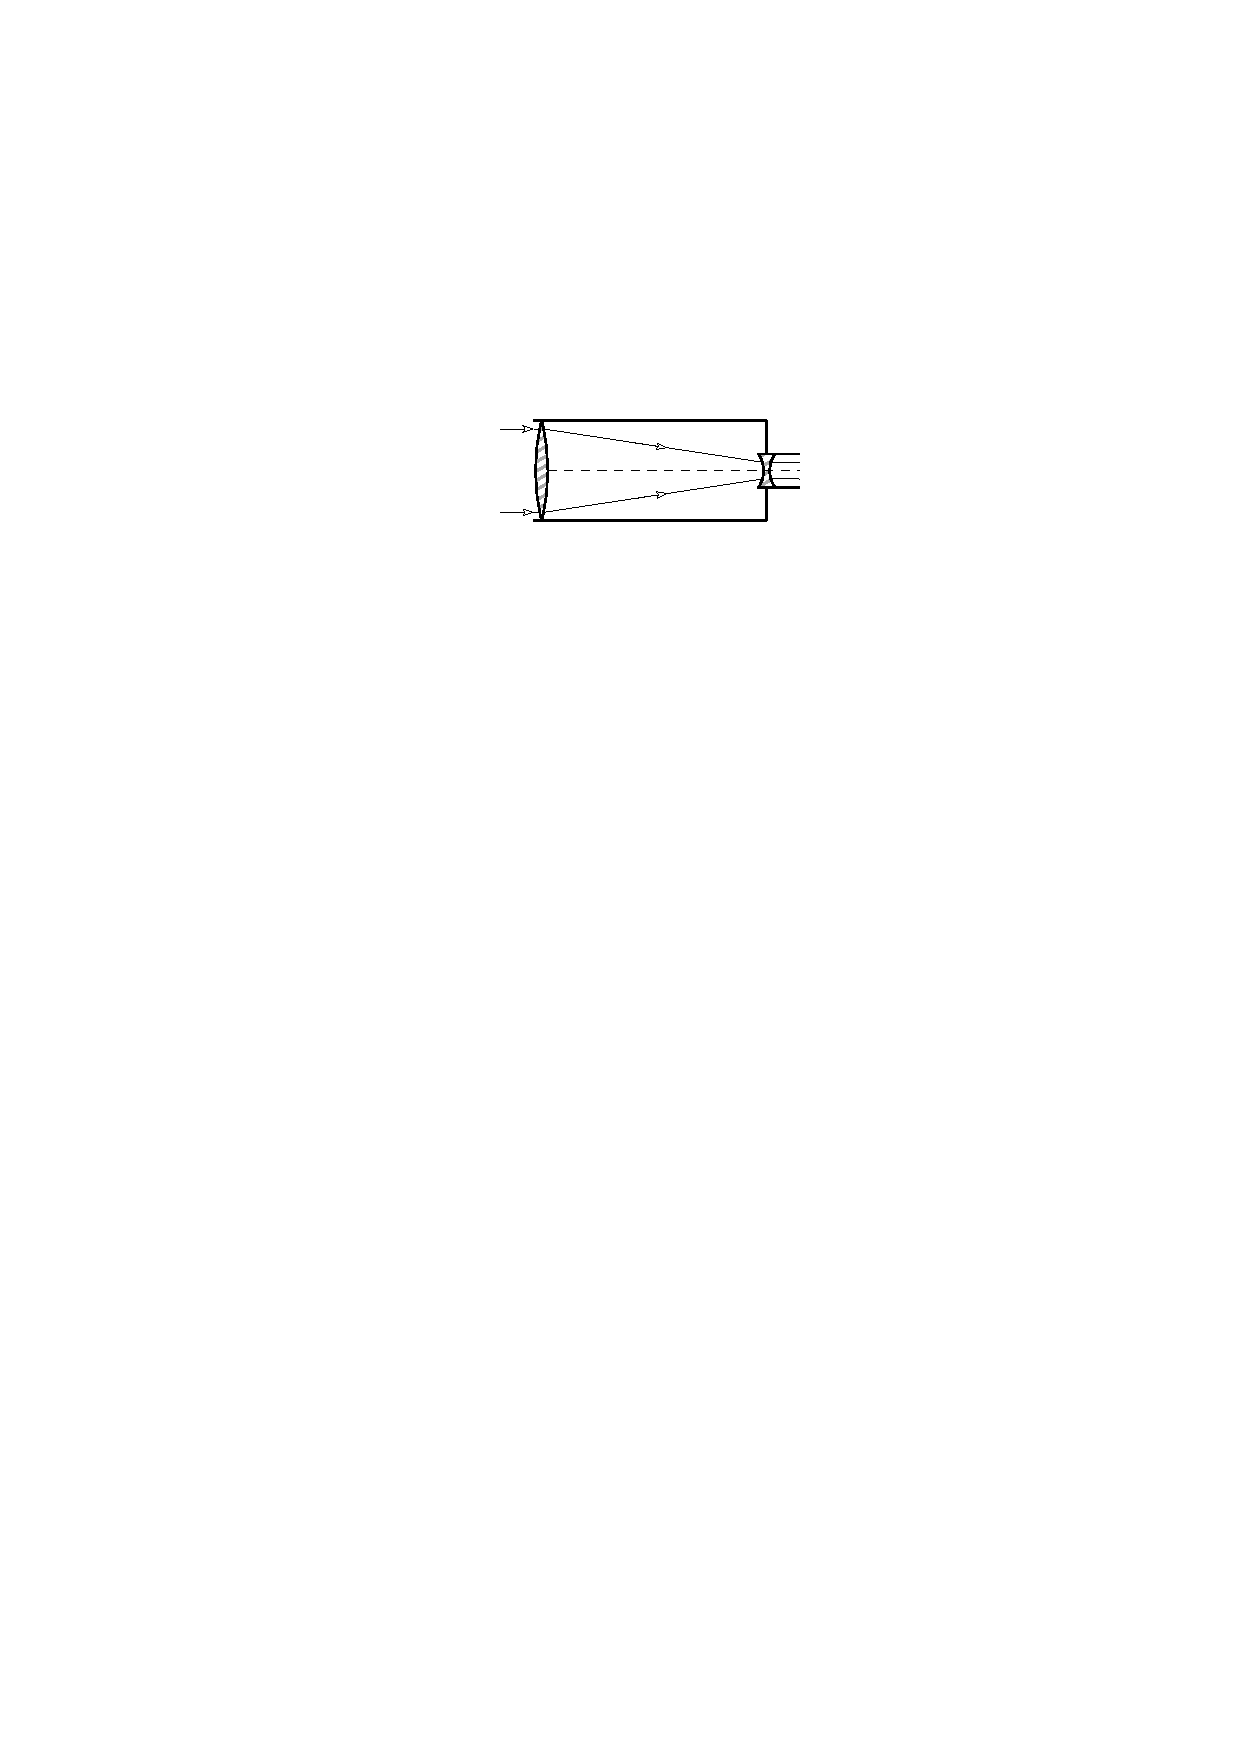
\includegraphics[width = \tw]{Galiley}
		\caption{\textit{Рефрактор системы Галилея}}
	 \end{subfigure}
	 \hfill
	\begin{subfigure}{0.49\tw}
		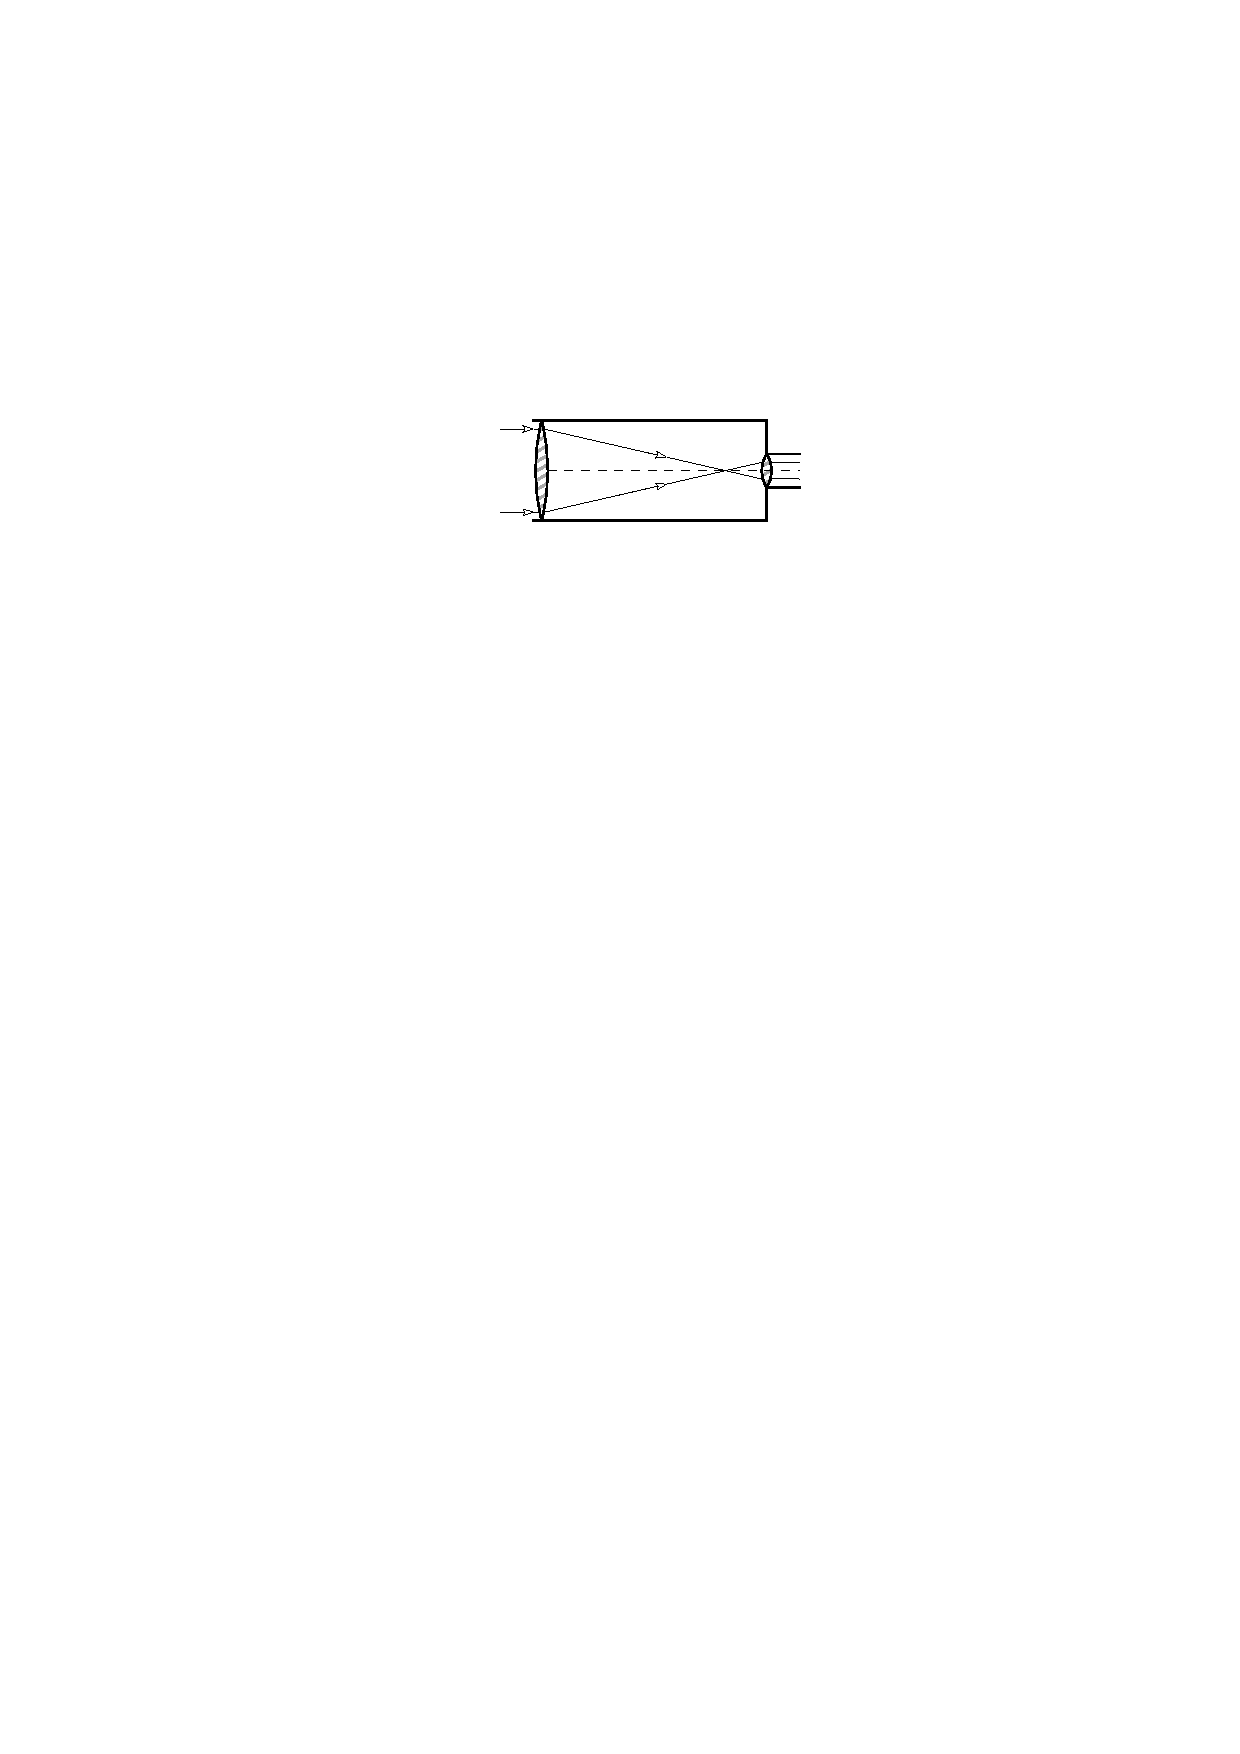
\includegraphics[width = \tw]{Kepler}
		\caption{\textit{Рефрактор системы Кеплера} \label{Kepler}}
	 \end{subfigure}
	 \vskip4pt
	 \begin{subfigure}{0.49\tw}
		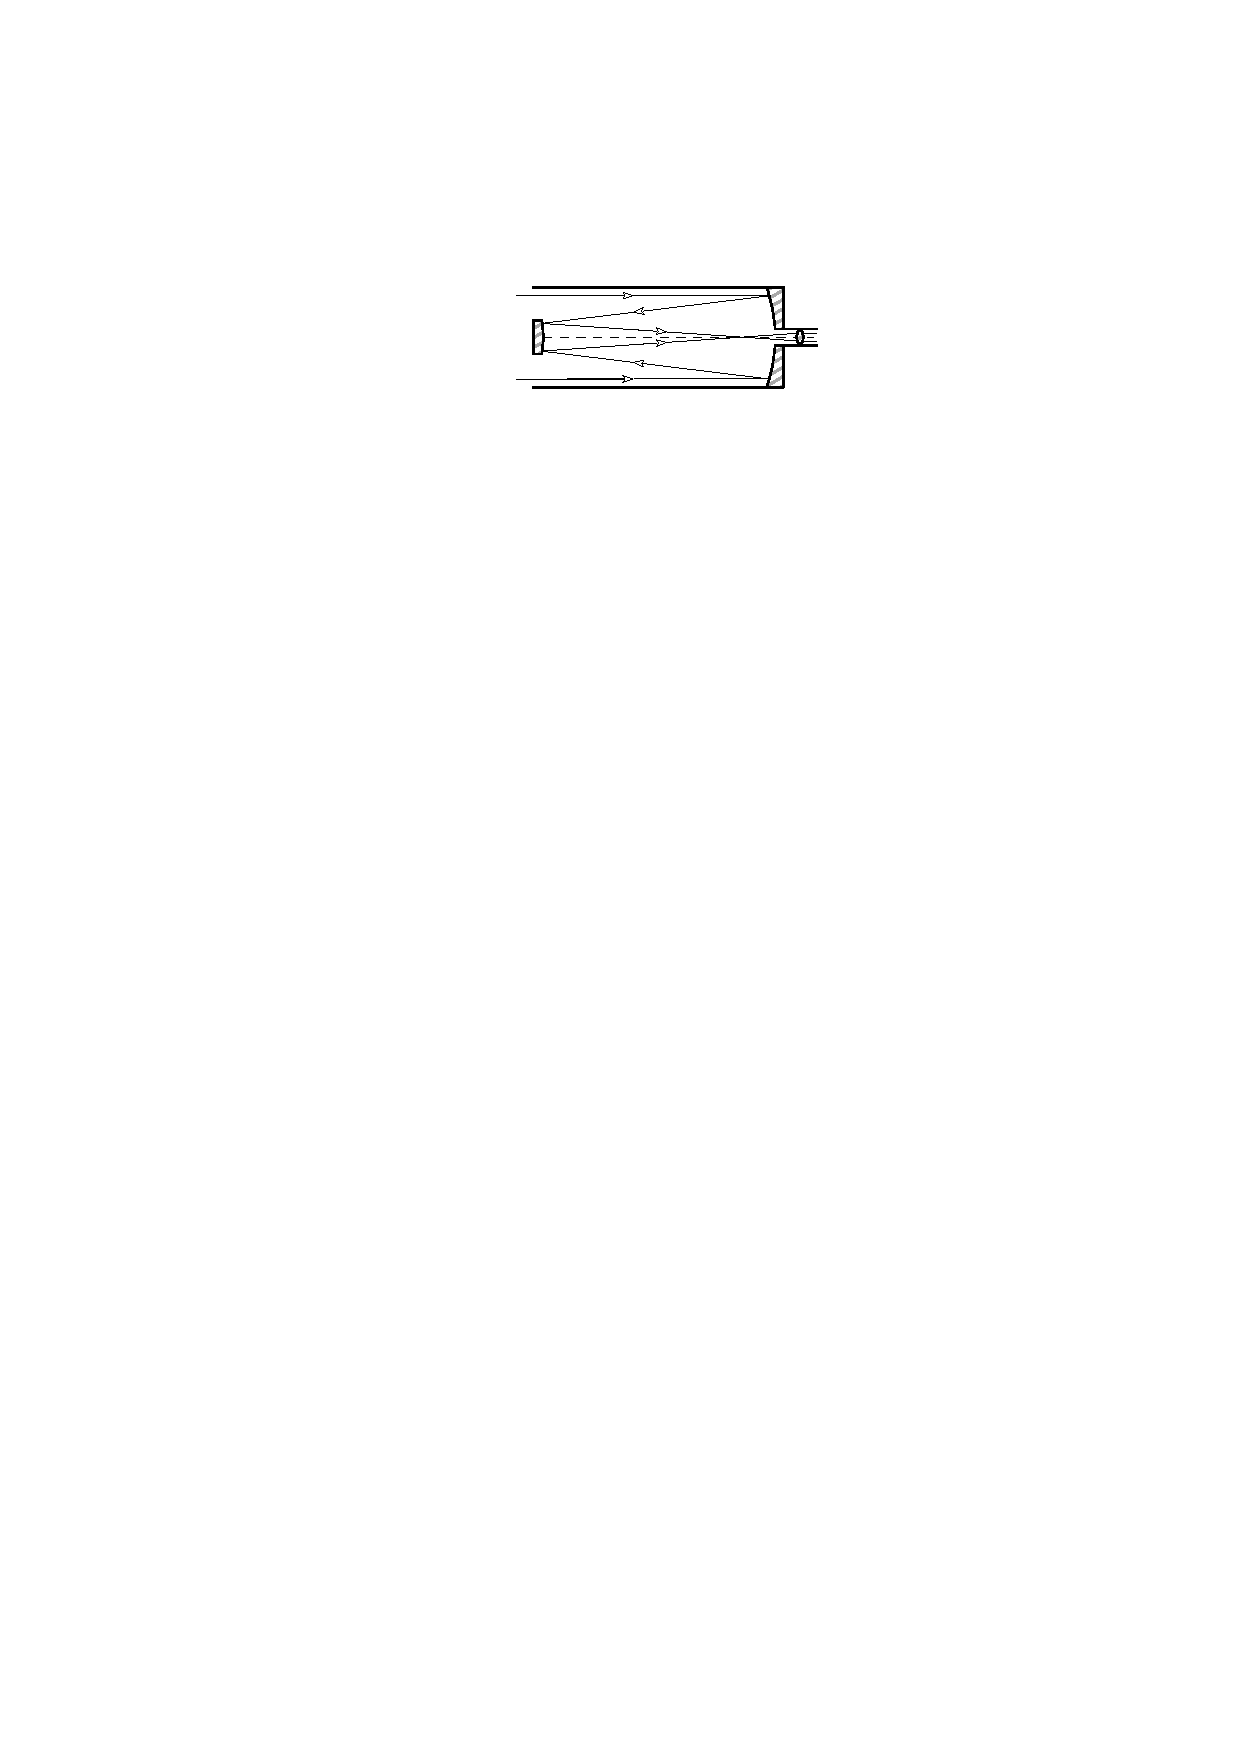
\includegraphics[width = \tw]
	{Cassigren.pdf}
	\caption{\textit{Рефлектор системы Кассигрена}}
	 \end{subfigure}
	 \hfill
	 \begin{subfigure}{0.49\tw}
		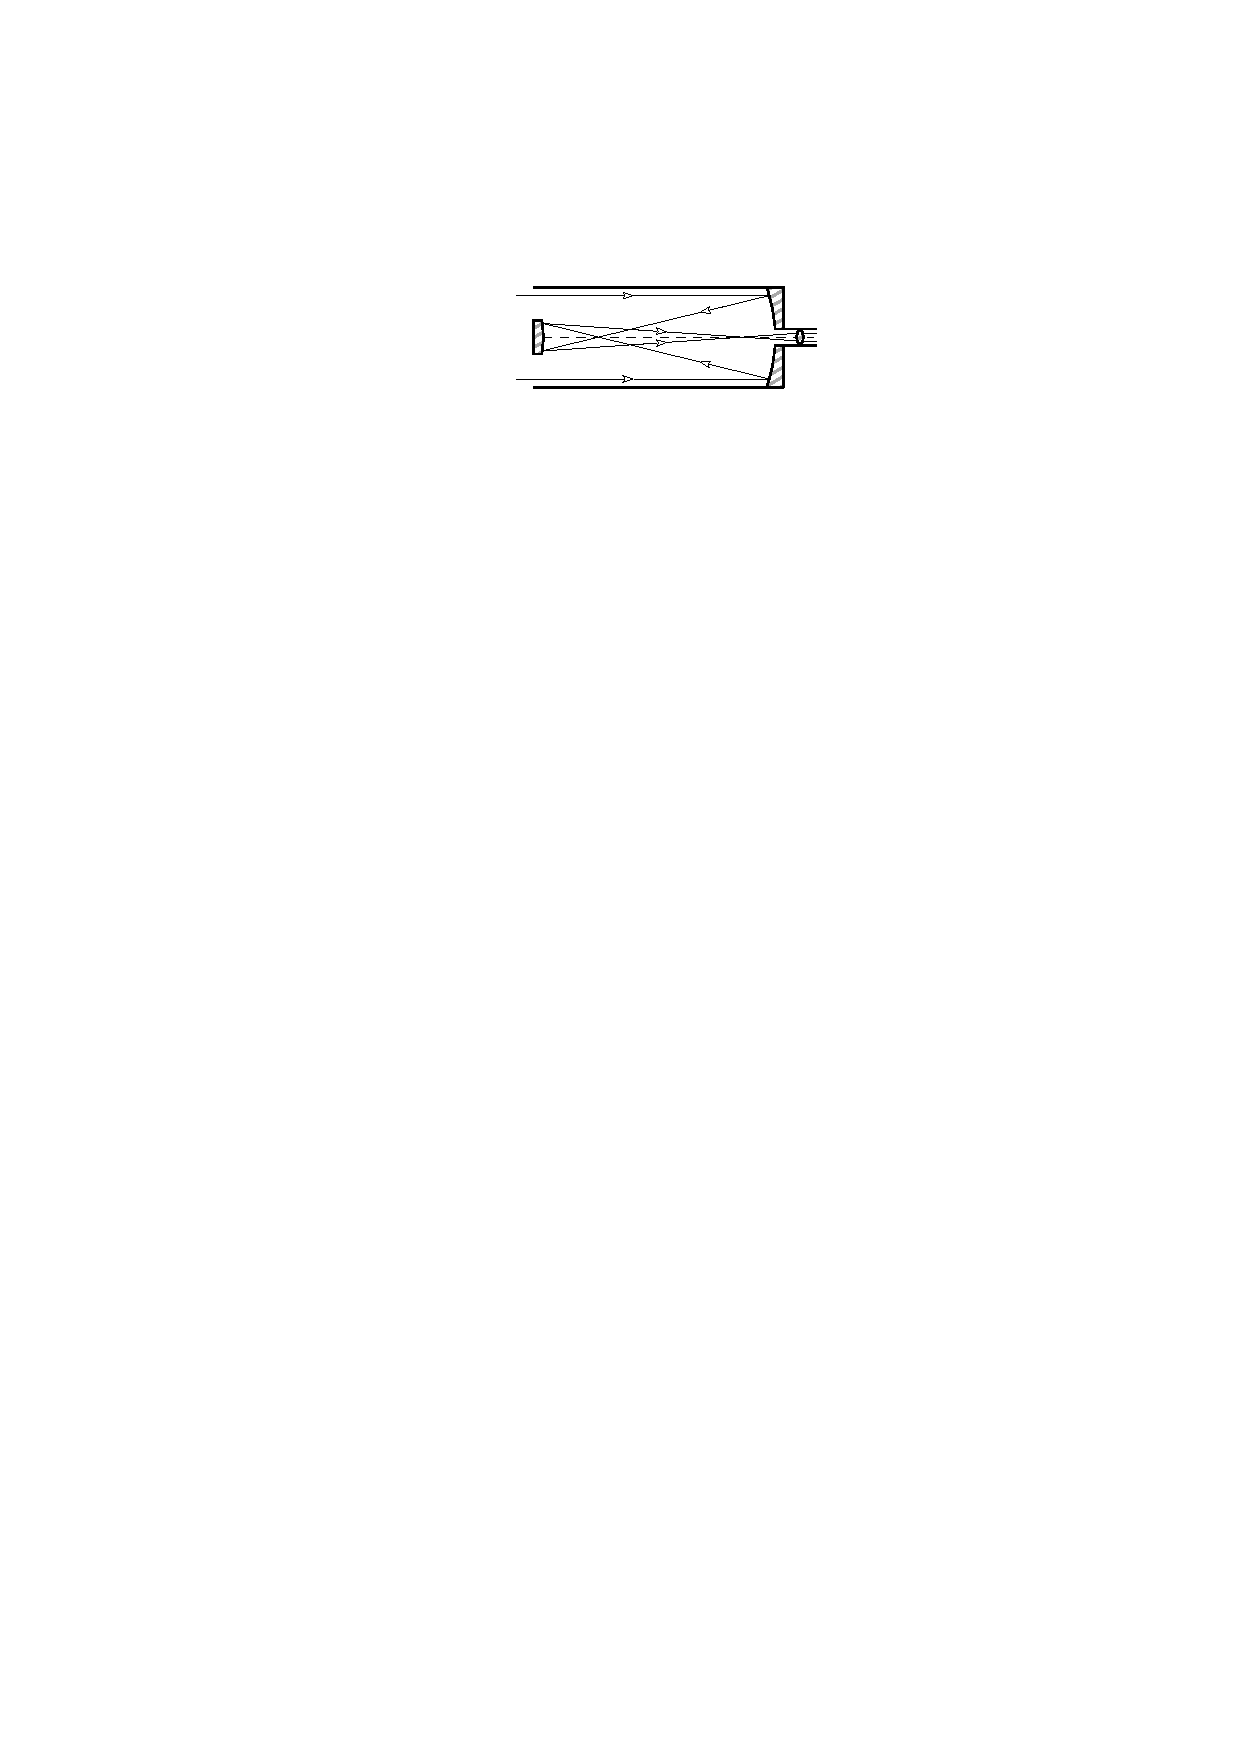
\includegraphics[width = \tw]
	{Gregory.pdf}
	\caption{\textit{Рефлектор системы Грегори} \label{Gregory}}
	 \end{subfigure}
	 \vskip4pt
	\begin{subfigure}{0.49\tw}
		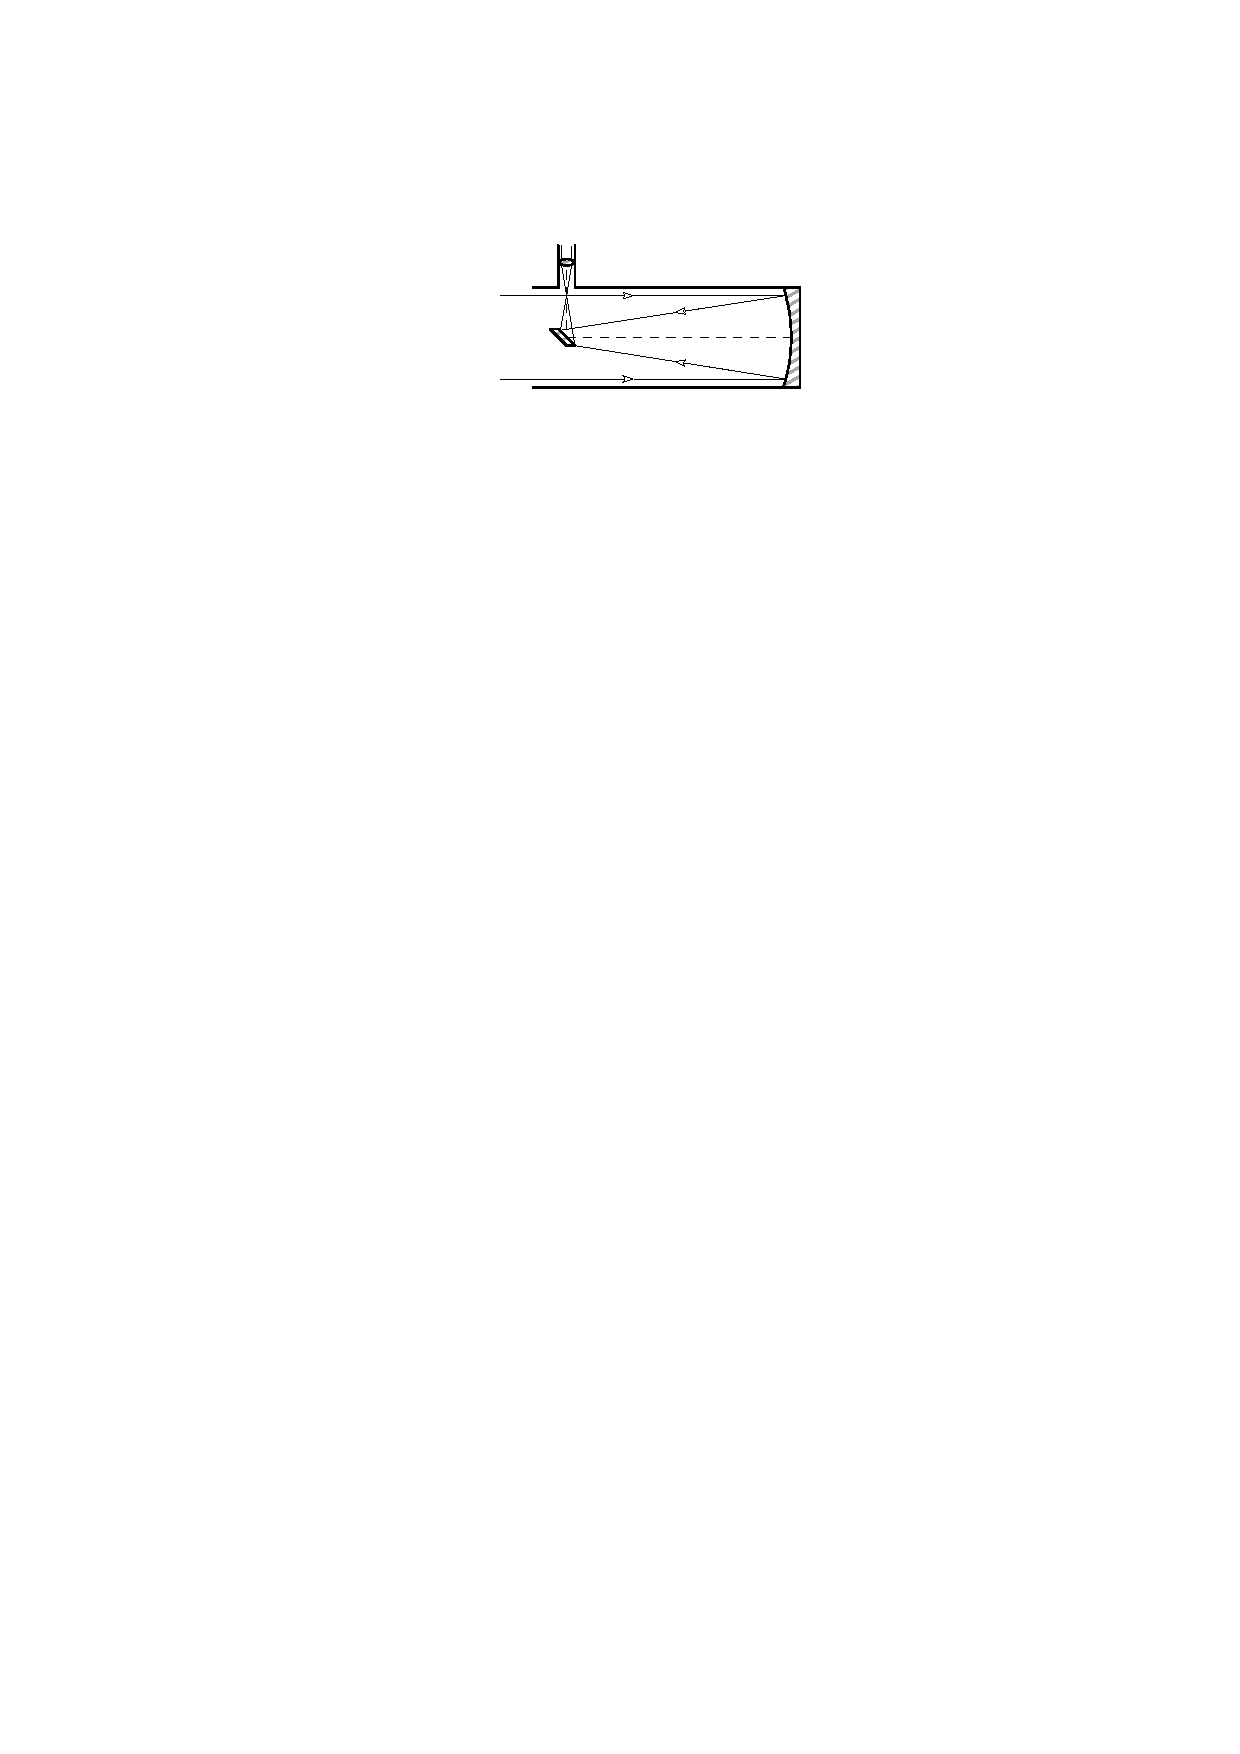
\includegraphics[width = \tw]
	{Newton.pdf}
	\caption{\textit{Рефлектор системы Ньютона} \label{Newton}}
	 \end{subfigure}
	 \hfill
	  \begin{subfigure}{0.49\tw}
		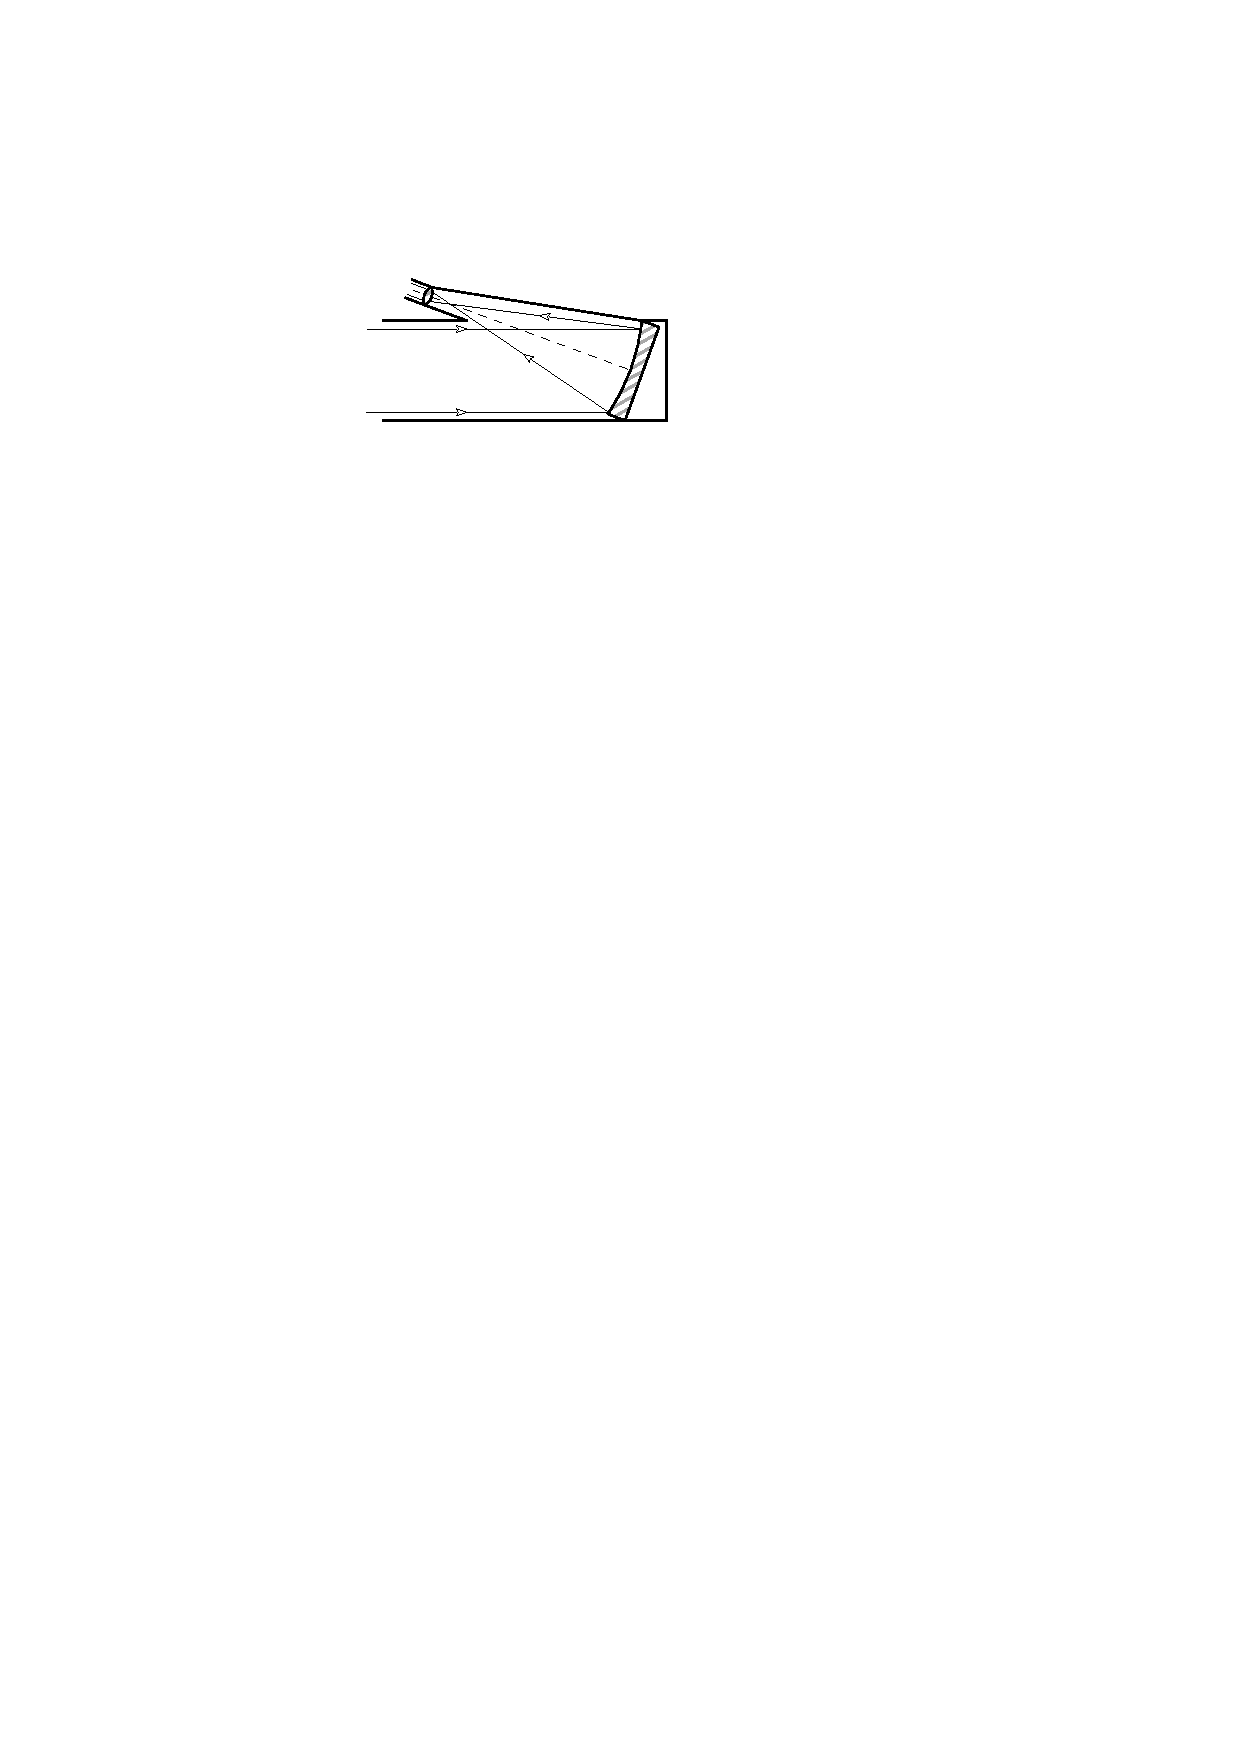
\includegraphics[width = \tw]
	{Lomonosov.pdf}
	\caption{\textit{Рефлектор системы Ломоносова}}
	 \end{subfigure}
	 
	
\end{figure}